\documentclass[border=4pt]{standalone}
\usepackage{fontspec}
\usepackage{amsmath}
\usepackage{unicode-math}
\setmainfont{Latin Modern Roman}
\setmathfont{Latin Modern Math}
\usepackage{pgfplots}
\usepackage{pgfplotstable}
\pgfplotsset{compat=1.18}
\usepackage{tkz-euclide}
\usetikzlibrary{arrows.meta,calc,angles,quotes,patterns,3d,backgrounds}
\definecolor{ink}{HTML}{123428}
\definecolor{asy}{HTML}{475569}
\definecolor{mint}{HTML}{86e0bd}
\tikzset{asym/.style={asy, line width=0.9pt, dash pattern=on 5pt off 3.5pt},
         guide/.style={gray!70, line width=0.6pt, densely dotted},
         dot/.style={circle, inner sep=0pt, minimum size=5pt, draw=white, line width=0.5pt},
         odot/.style={circle, inner sep=0pt, minimum size=5.5pt, fill=white, line width=1pt},
         lab/.style={font=\footnotesize, inner sep=1.5pt, text=ink}}
\begin{document}
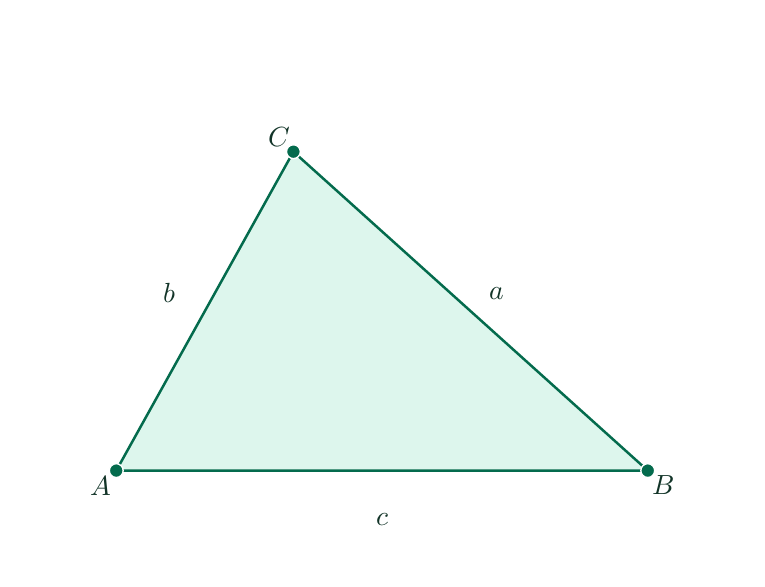
\begin{tikzpicture}[x=1.1250cm, y=1.1250cm]
\tkzDefPoint(0,0){A}
\tkzDefPoint(6,0){B}
\tkzDefPoint(2,3.6){C}
\begin{scope}
\clip (-1,-1) rectangle (7,5);
\tkzFillPolygon[fill={rgb,255:red,134;green,224;blue,189}, fill opacity=0.28](A,B,C)
\tkzDrawPolygon[draw={rgb,255:red,4;green,107;blue,77}, line width=0.9pt](A,B,C)
\end{scope}
\node[dot, fill={rgb,255:red,4;green,107;blue,77}] at (A) {};
\node[dot, fill={rgb,255:red,4;green,107;blue,77}] at (B) {};
\node[dot, fill={rgb,255:red,4;green,107;blue,77}] at (C) {};
\node[lab, font=\normalsize] at (3,-0.55) {$c$};
\node[lab, font=\normalsize] at (4.3,2) {$a$};
\node[lab, font=\normalsize] at (0.6,2) {$b$};
\node[lab, font=\normalsize, anchor=north east] at (0,0) {$A$};
\node[lab, font=\normalsize, anchor=north west] at (6,0) {$B$};
\node[lab, font=\normalsize, anchor=south east] at (2,3.6) {$C$};
\end{tikzpicture}
\end{document}
